\documentclass[a4paper,12pt]{article}

% Package Imports
\usepackage{styles/ibu-thesis} % Ensure this file exists in your directory
\usepackage{subcaption}
\usepackage{graphicx}
\usepackage{float}
\usepackage[export]{adjustbox}
\usepackage[all]{nowidow} 
\usepackage{booktabs} 
\usepackage{array}
\usepackage{cite} 
\usepackage{enumitem}
\usepackage{tikz} 
\usetikzlibrary{shapes.geometric, shapes.misc, shapes.symbols, arrows.meta, positioning, fit, backgrounds, calc, decorations.pathreplacing}

\definecolor{orbisInk}{HTML}{1F2933}
\definecolor{orbisBlue}{HTML}{2563A9}
\definecolor{orbisTeal}{HTML}{0F766E}
\definecolor{orbisGold}{HTML}{B7791F}
\definecolor{orbisRed}{HTML}{B42318}
\definecolor{orbisGreen}{HTML}{2F855A}
\definecolor{orbisPanel}{HTML}{F7FAFC}
\definecolor{orbisLine}{HTML}{CBD5E1}

% Formatting for cleaner structure and paragraph gaps
\setlength{\parindent}{0pt}   
\setlength{\parskip}{5px}     

% STRUCTURAL FIXES
\raggedbottom
\clubpenalty=10000
\widowpenalty=10000

% Thesis Title
\thesistitle{Orbis: An Intelligent Academic Support System with AI and RAG}

% Author Information
\authors[1]{Atakan Gül}
\authorsid[1]{121200152}
\authors[2]{Arda Kaan Y{\i}ld{\i}z}
\authorsid[2]{122200045}

% Supervisor Information
\supervisors[1]{Özgür Özdemir}

% Affiliation Information
\faculty{Faculty of Engineering and Natural Sciences}
\degree{Bachelor of Science}
\department{Department of Computer Engineering}
\submissiondate{June, 2026} 

\abstract{
University academic systems often function merely as static record-keeping databases, lacking proactive support for students navigating complex degree requirements. This project, 'Orbis', introduces an intelligent academic support system designed to bridge this gap using Artificial Intelligence (AI) and Retrieval-Augmented Generation (RAG). The core of Orbis is an Orchestrator-led event management pipeline that autonomously monitors a student's dynamic academic state against a complex vector database of university regulations, triggering timely notifications for critical milestones. To achieve high fidelity, we engineered a taxonomy generation pipeline utilizing Shannon entropy tail-signal classification and MiniBatchKMeans clustering, organizing 60,649 document chunks into 125 high-quality leaf nodes. Our pipeline features a two-pass adversarial LLM review, evaluating 323 candidate rules and extracting 178 highly actionable obligations with a 55\% acceptance rate, and matches them against 4 distinct student profiles to generate 176 personalized assignments. We evaluate each subsystem against a gold ground-truth set manually validated by the authors. The event-extraction stage achieves precision 0.978 / recall 0.574 / $F_1$ 0.723 over 323 candidates; the assignment-matching stage achieves $F_1$ 0.51 over 712 (profile, obligation) pairs. An agentic submission-review subsystem evaluated on 32 deterministically generated cases attains 93.8\% accuracy with perfect recall and full ($4/4$) resistance to in-document prompt injection. Complementing the event and submission systems, a production-grade RAG chatbot enables natural-language queries over the full institutional knowledge base; evaluated against a 100-query bilingual benchmark across seven routing categories, it achieves 92\% routing accuracy, 95\% context recall, a Mean Reciprocal Rank of 0.94, and 98\% semantic accuracy. The remaining roadmap includes direct integration with the university's Student Information System (SIS) and injection-hardened submission review.
}

\begin{document}

% Preliminaries
\maketitle
\addcontentsline{toc}{section}{\abstractname}
\makeabstract
\addcontentsline{toc}{section}{\contentsname}
\maketableofcontents

\addcontentsline{toc}{section}{List of Figures}
\makelistoffigures
\addcontentsline{toc}{section}{List of Tables}
\makelistoftables

% List of abbreviations
\addcontentsline{toc}{section}{\listofabbrv}
\makelistofabbrv
\begin{abbrv}
    \item[AI] Artificial Intelligence
    \item[API] Application Programming Interface
    \item[CI/CD] Continuous Integration/Continuous Deployment
    \item[DB] Database
    \item[GIN] Generalized Inverted Index
    \item[HAC] Hierarchical Agglomerative Clustering
    \item[HNSW] Hierarchical Navigable Small World
    \item[LLM] Large Language Model
    \item[MRR] Mean Reciprocal Rank
    \item[RAG] Retrieval-Augmented Generation
    \item[SIS] Student Information System
    \item[SSE] Server-Sent Events
    \item[TF-IDF] Term Frequency-Inverse Document Frequency
\end{abbrv}
\newpage

\pagenumbering{arabic}
\setcounter{page}{1}

% Sections
\section{Introduction}
In universities, students face a significant cognitive load managing complex degree rules, course selections, and deadlines. Traditional academic platforms are often designed as static databases. They store information efficiently but fail to interpret it for the student's benefit. Students generally do not miss deadlines because they cannot search a system; they miss them because they do not know what they are supposed to be looking for. This creates a "synchronization gap" between student needs and institutional data.

Our project, 'Orbis', offers a novel solution by shifting the academic paradigm from static storage to autonomous orchestration. Orbis is built to act as a proactive academic agent operating through two tightly integrated subsystems. The \textbf{Proactive Event System} autonomously evaluates a student's specific academic state against unstructured university regulations to trigger unprompted, obligation-based notifications. The \textbf{RAG Chatbot} complements this by enabling students and faculty to interactively query the same institutional knowledge base in natural language---answering questions about regulations, course catalogs, academic calendars, and personal timetables in real time.

Crucially, the architecture of Orbis is designed for scalability. The system relies on a strictly orchestrated workflow to execute its primary use case: the \textbf{Proactive Event System}. This autonomous pipeline extracts strict, assignable obligations from regulatory documents and creates normalized events, allowing the system to trigger timely, unprompted notifications for students regarding their specific academic requirements.

The rest of the work is organized as follows. Section 2 overviews related works. Section 3 details the dataset. Section 4 provides the theoretical background. Section 5 presents the proposed methodology, covering the event pipeline, submission agent, and RAG chatbot architecture. Section 6 describes the experimental setup. Sections 7 and 8 discuss experiments and results. Section 9 provides quantitative evaluation. Section 10 concludes the paper.

\section{Related Works}
Academic support systems have evolved from static record-keeping into AI-mediated tools, but most existing systems remain reactive: they answer student questions but do not autonomously enforce regulations against a student's state. We position Orbis against seven lines of work.

\textbf{RAG-based academic chatbots.} Retrieval-Augmented Generation combines a generative LLM with a non-parametric retrieval store, grounding answers in source documents and reducing hallucination \cite{lewis2020retrieval}. A systematic review of advising chatbots screened 128 studies and retained 11 advising-chatbot papers, finding that most systems target admission or academic-advising dialogue rather than autonomous obligation enforcement \cite{assayed2024systematic}. More recent advising-LLM work reports QA-style metrics such as BLEU, ROUGE-L, and student satisfaction ratings \cite{ismail2025academic}. These systems serve well as on-demand search interfaces, but operate strictly in a pull mode --- a student must already know that a question is worth asking. Orbis instead operates in a push mode: it parses regulations into structured obligations and matches them against profiles before the student asks.

\textbf{Degree-audit systems.} Tools such as DegreeWorks and Stellic encode degree requirements as deterministic rules and audit a transcript against them. The Degree Audit Reporting System (DARS), for example, has been studied as an advising and registration-support system rather than as an information-extraction benchmark \cite{wick2023dars}. Such systems are excellent for objective conditions (credit counts, GPA thresholds) but cannot reason about unstructured policy text (procedural requirements, deadline-bearing obligations, exceptions written in prose). Orbis complements deterministic audit with a contextual LLM path that operates over free-text regulation.

\textbf{Regulatory information extraction.} Prior regulatory IE work is closer to Orbis's event-extraction subsystem, but not to the full Orbis pipeline. Zhang and El-Gohary report 0.969 precision and 0.944 recall when extracting quantitative requirements from the 2009 International Building Code using semantic NLP rules \cite{zhang2016semantic}. Recent legal-obligation extraction work on the EU AI Act reports 93\% precision for obligation filtering and over 99\% accuracy for classifying obligation type, addressee, and predicate \cite{galli2025aiAct}. These results are useful precision/recall comparators for the extraction stage, but their domains, source documents, and output schemas differ from university-student obligation assignment.

\textbf{Local context: HermiOne.} Istanbul Bilgi University has deployed ``HermiOne,'' a support chatbot built by the university's IT department. Based on publicly observable behavior at the time of writing, HermiOne appears to operate primarily as a reactive question-answering chatbot rather than as a proactive regulation-enforcement agent; a direct comparison would require access to its design documentation, which we did not have. Orbis is intentionally complementary: HermiOne handles the conversational interface, while Orbis produces the underlying structured event stream that a future iteration of HermiOne could subscribe to.

\textbf{Hybrid retrieval and neural re-ranking.} A consistent finding in the RAG literature is that dense vector search alone is insufficient when the target corpus is large and heterogeneous: exact-term queries benefit disproportionately from sparse keyword retrieval. Hybrid approaches that interleave BM25-style inverted-index results with dense vector results before a final re-ranking step have been shown to outperform either method in isolation across domain-specific corpora \cite{kiela2024hybrid}. Beyond retrieval, cross-encoder re-rankers---which score (query, document) pairs jointly rather than encoding them independently---substantially improve precision when applied to the candidate pool before it reaches the generative model \cite{gunther2023jina}. The Orbis RAG chatbot implements both of these findings as load-bearing components rather than optional optimizations.

\textbf{Automated submission assessment.} LLM-assisted grading systems provide a useful comparison point for the submission-review subsystem, but their metrics usually measure grade prediction rather than safety-oriented accept/reject screening. JorGPT, for instance, evaluates programming-assignment grading over 672 submissions and reports adjusted $R^2{=}0.9156$, mean absolute error $0.4579$, and a reduction from over 300 hours of manual work to under 15 minutes of automated processing \cite{cisneros2025jorgpt}. Orbis's submission agent is narrower: it does not assign grades, but checks whether a submitted artifact satisfies assignment requirements and preserves an appeal path.

\textbf{LLM-as-a-judge for evaluation.} Because labeled gold sets for university-specific regulation extraction do not exist publicly, we adopt the LLM-as-a-judge methodology \cite{zheng2023judging}, in which an independent LLM is used as a scalable proxy for human labeling and validated against a second model from a different family. This methodology underlies our evaluation in Section~9.

Table~\ref{tab:related_work} summarizes the comparison.

\begin{table}[H]
\centering
\small
\begin{tabular}{lcccc}
\toprule
System type & Pull/push & Unstructured rules & Student-specific & Auto-notify \\ \midrule
University FAQ chatbot     & Pull & No  & No  & No  \\
RAG academic chatbot       & Pull & Yes & No  & No  \\
Deterministic degree audit & Push & No  & Yes & Partial \\
HermiOne (reactive)        & Pull & Yes & Partial & No \\
\textbf{Orbis (this work)} & \textbf{Push} & \textbf{Yes} & \textbf{Yes} & \textbf{Yes} \\
\bottomrule
\end{tabular}
\caption{Positioning of Orbis against related categories of academic-support systems. \emph{Push} means the system surfaces an obligation before a student asks. \emph{Unstructured rules} means handling free-text regulation, not only schema-based requirements.}
\label{tab:related_work}
\end{table}

No exact end-to-end baseline was found for the combined task Orbis addresses: proactive extraction of university regulations, profile-specific obligation assignment, and submission review with appeal. Therefore, Table~\ref{tab:baseline_validity} compares Orbis against official prior work at the subsystem level and explicitly marks whether each comparison is direct, partial, or contextual. This distinction is important: we do not claim that Orbis ``beats'' systems evaluated on different tasks; we use them to position the contribution and to choose defensible metrics.

\begin{table}[H]
\centering
\scriptsize
\begin{adjustbox}{width=\textwidth}
\begin{tabular}{>{\raggedright\arraybackslash}p{3.2cm}>{\raggedright\arraybackslash}p{2.5cm}>{\raggedright\arraybackslash}p{3.4cm}>{\raggedright\arraybackslash}p{2.2cm}>{\raggedright\arraybackslash}p{4.7cm}}
\toprule
\textbf{Official prior work} & \textbf{Related Orbis subsystem} & \textbf{Reported metric or scope} & \textbf{Comparison type} & \textbf{How it is used in this report} \\ \midrule
Assayed et al. systematic review \cite{assayed2024systematic} & Advising-chatbot landscape & 128 articles screened; 11 included advising-chatbot studies & Contextual & Shows that advising chatbots are active research systems, but mostly dialogue/admission/advising tools rather than proactive rule-assignment pipelines. \\
Ismail academic-advising LLM \cite{ismail2025academic} & Advising chatbot & BLEU 0.45$\rightarrow$0.78; ROUGE-L 0.85; 50-student ratings 4.6--4.8/5 & Contextual & Provides QA-chatbot metrics; not directly compared because Orbis is evaluated on extraction, matching, and submission screening rather than answer generation. \\
Wick and Wallingford DARS study \cite{wick2023dars} & Degree audit & Qualitative analysis of DARS for advising and registration support & Contextual & Positions deterministic degree-audit systems as complements, not direct NLP baselines. \\
Zhang and El-Gohary regulatory IE \cite{zhang2016semantic} & Event extraction & Precision 0.969; recall 0.944 on building-code quantitative requirements & Partial & Provides a precision/recall comparator for regulatory extraction, with different domain and rule schema. \\
Galli et al. AI Act obligation extraction \cite{galli2025aiAct} & Event extraction & 93\% obligation-filtering precision; $>$99\% classification accuracy for extracted obligation fields & Partial & Provides a modern legal-obligation extraction comparator; not compared to assignment matching or submission review. \\
JorGPT LLM grading \cite{cisneros2025jorgpt} & Submission assessment & Adjusted $R^2$ 0.9156; MAE 0.4579; 672 submissions; 300+ hours $\rightarrow$ under 15 minutes & Partial & Provides grading/workload context; Orbis reports binary accept/reject safety metrics instead of grade-regression metrics. \\
Prior Orbis single-call reviewer & Submission review & Accuracy 0.781; injection resistance 1/4 & Direct & Internal ablation baseline for the current two-call reviewer reported in Section~9.4. \\
\bottomrule
\end{tabular}
\end{adjustbox}
\caption{Official baseline and comparator validity. \emph{Direct} means the same task and data family; \emph{partial} means a related subsystem metric but different domain or output schema; \emph{contextual} means useful for positioning only.}
\label{tab:baseline_validity}
\end{table}

\section{Dataset}
The foundation of Orbis is its institutional \texttt{knowledge\_base}, constructed from 80 official source URLs under the \texttt{bilgi.edu.tr} domain. The dataset and its post-processing artifacts are summarized in Table~\ref{tab:dataset_stats}.

\begin{table}[H]
\centering
\begin{tabular}{lr}
\toprule
Quantity & Value \\ \midrule
Source URLs crawled & 80 \\
Raw document chunks & 60{,}649 \\
Languages observed & English, Turkish \\
Top-level taxonomy categories (LLM-mapped) & 11 \\
Leaf-level taxonomy nodes & 125 \\
Regulatory leaves (post-overlay) & 29 \\
Regulatory chunks (event-pipeline input) & 935 \\
Accepted obligations (\texttt{regulation\_rules}) & 178 \\
Student profiles (\texttt{user\_profiles}) & 4 \\
\bottomrule
\end{tabular}
\caption{Dataset and post-processing statistics. The Proactive Event System operates only on the 935 regulatory chunks; all other categories are routed to the RAG search index.}
\label{tab:dataset_stats}
\end{table}

The crawl is intentionally heterogeneous: it contains formal regulations (student handbooks, dual-major directives, internship procedures), administrative announcements, event pages, and upload directories. The corpus is bilingual, which complicates deduplication --- the same regulation often exists under both \texttt{/en/academics/...} and \texttt{/tr/akademik/...} paths. Chunking is performed at ingest time using a semantic splitter with a soft 800-token target and a 100-token overlap; each chunk is embedded once with a local MiniLM model and stored in \texttt{knowledge\_base\_embeddings} alongside the source URL, content hash, and categorical metadata. The regulation subset is isolated via the four-step taxonomy pipeline of Section~5.1, with a final regex overlay that promotes any chunk whose source URL matches a known regulation path into the \texttt{regulation} or \texttt{regulation\_document} category, preventing event-pipeline cross-contamination from non-binding content. Instead, evaluation is performed against a constructed Gold Ground-Truth testing set, detailed in Section~9.

\subsection{RAG Knowledge Base Preparation}
\label{sec:rag_dataset}

The same \texttt{knowledge\_base} table serves as the retrieval index for the RAG chatbot, but the full chatbot-facing corpus has a substantially broader scope than the 935-chunk regulatory subset consumed by the event pipeline. Understanding its structure is necessary to explain several design decisions in the retrieval architecture.

\textbf{Web page distribution.} Approximately 12,600 web pages were scraped from the university domain. Table~\ref{tab:web_distribution} shows the category breakdown.

\begin{table}[H]
    \centering
    \begin{adjustbox}{center}
        \begin{tabular}{l c c p{5.5cm}}
            \toprule
            \textbf{Category} & \textbf{Count} & \textbf{Share} & \textbf{Description} \\ \midrule
            News \& Announcements & $\approx$4,160 & 33\% & Press releases, news items (\texttt{/haber/}) \\
            Events                & $\approx$4,035 & 32\% & Past and future seminars (\texttt{/etkinlik/}) \\
            Academic (Faculties)  & $\approx$2,268 & 18\% & Department pages, faculty bios, course lists \\
            University Info       & $\approx$1,008 &  8\% & Rules, administration, ``About Us'' pages \\
            Student Life          & $\approx$630   &  5\% & Transport, clubs, support services \\
            Other                 & $\approx$507   &  4\% & International office, research centers \\
            \bottomrule
        \end{tabular}
    \end{adjustbox}
    \caption{Web Page Corpus Distribution by Category}
    \label{tab:web_distribution}
\end{table}

65\% of the corpus is \textit{temporal} content (news and event pages), while only $\approx$35\% is \textit{core knowledge}. This imbalance is the primary retrieval challenge: a na\"{i}ve vector search for ``scholarship policy'' risks surfacing a 2018 news article announcing a policy update rather than the current policy page. The router architecture (Section~5.5) addresses this by steering factual queries away from high-temporal URL prefixes.

\textbf{PDF filtering.} Approximately 2,245 scraped PDFs were analyzed. Construction tenders (\texttt{/ihaleler/}) use legalistic language (``Article 5'', ``Obligations'') that semantically overlaps with academic regulations; recruitment result lists contain thousands of proper nouns and scores that dilute the vector space. A \texttt{filter\_pdfs.py} script applied hard-exclusion rules by URL pattern and Turkish keyword (e.g.\ ``teklif mektubu''---Proposal Letter; ``sonuç listesi''---Result List), with hard-inclusion overrides protecting known high-value documents (any file containing ``erasmus'', ``staj'', ``handbook'', or ``yönerge'' is always retained). The result: \textbf{1,595 files ingested} (regulations, syllabuses, Erasmus guides, brochures), \textbf{315 discarded} (tenders, outdated recruitment lists), and \textbf{335 archived} (faculty CVs, reserved for a future Faculty Search feature).

\textbf{Language detection.} Accurate language tagging drives correct PostgreSQL stemming in the TSVector search index. A simple character-frequency heuristic (counting Turkish-specific characters such as \texttt{\i, ğ, ş}) failed on English documents containing local addresses (e.g., ``Santral Campus, Eyüpsultan''). The adopted approach runs a \textit{Stopword Race}: it counts occurrences of language-specific stopwords (\textit{the, and, is} vs.\ \textit{ve, bir, için}) over the document body, resolving language from content rather than character inventory. A \texttt{fix\_pdf\_language\_and\_titles.py} preprocessing step repaired \textbf{361 PDF titles} (22.6\% of the corpus) that carried generic software-generated names (e.g., ``PowerPoint Presentation''), falling back to a clean title derived from the filename. Final language split: $\approx$65\% Turkish, $\approx$35\% English.

\section{Theoretical Background}
To successfully isolate and evaluate this dataset, Orbis relies on several foundational machine learning and information theory algorithms. 

\subsection{Shannon Entropy for URL Classification}
To classify opaque URL structures, we measure the diversity of URL "tails" using Shannon Entropy \cite{shannon1948mathematical}. A high entropy value indicates that a URL directory is semantically informative, whereas low entropy implies repetitive or dynamic templates.
$$H = -\sum_{i=1}^{n} p_i \cdot \log_2(p_i)$$
Where $p_i$ is the probability of a specific URL pattern occurring within a given parent group.

\subsection{Vector Embeddings and Cosine Similarity}
Text chunks are transformed into high-dimensional numerical vectors. To measure the semantic similarity between two chunks (or a user query and a document), we calculate the Cosine Similarity.
$$\cos(\theta) = \frac{\mathbf{A} \cdot \mathbf{B}}{\|\mathbf{A}\| \|\mathbf{B}\|}$$
Prior to clustering, we perform L2-Normalization on all vectors ($\hat{v} = \frac{v}{\|v\|}$), converting cosine distance into Euclidean distance on a unit sphere, optimizing it for K-Means processing.

\subsection{MiniBatchKMeans and Ward HAC}
For semantic discovery of opaque URLs, we deploy MiniBatchKMeans, which utilizes random mini-batches to achieve linear time complexity $\mathcal{O}(n)$ suitable for large datasets \cite{sculley2010web}. This is followed by Ward Hierarchical Agglomerative Clustering (HAC) on the centroids. Ward's method merges clusters to minimize the total within-cluster variance \cite{ward1963hierarchical}.

\subsection{Hybrid Retrieval and Neural Re-Ranking}
\label{sec:theory_hybrid}

The RAG chatbot relies on two complementary retrieval mechanisms executed in parallel before a cross-encoder re-ranking stage consolidates their outputs.

\textbf{Full-text keyword search} operates on a \texttt{TSVECTOR} column maintained by PostgreSQL as a \texttt{GENERATED ALWAYS AS \ldots{} STORED} computed expression. The column applies language-aware stemming---automatically selecting the Turkish or English lexical parser based on each row's \texttt{language} field---to both the document title (indexed at weight `A', higher priority) and the content body (weight `B'). Queries are converted to \texttt{tsquery} expressions using OR logic, ensuring that any single key term match surfaces the document. A GIN (Generalized Inverted Index) is maintained on this column to enable sub-millisecond full-text lookups at 60,000+ rows.

\textbf{Semantic vector search} queries a 384-dimensional \texttt{pgvector} embedding column using L2/Euclidean distance against an HNSW (Hierarchical Navigable Small World) graph index \cite{malkov2018hnsw}. HNSW enables approximate nearest-neighbor search with a configurable recall/speed trade-off; the L2 metric is an intentional implementation choice that performs well empirically with the selected MiniLM embedding model.

\textbf{Cross-encoder re-ranking} applies a neural model (\texttt{jina-reranker-v2-base-multilingual}) that scores each (query, document) pair \textit{jointly}, capturing relevance nuances that a bi-encoder---which encodes query and document independently into fixed vectors---cannot. Cross-encoders are computationally expensive and therefore impractical for initial retrieval over large corpora, but highly effective when applied to the smaller candidate pool produced by hybrid search. The Orbis chatbot applies this step \textit{twice} in a two-stage architecture described in Section~5.5.

\section{Proposed Methodology}
The Orbis architecture is divided into three major components: Data Categorization (Taxonomy), the Orchestrator-led Event Pipeline, and the RAG Chatbot.

\subsection{Data Categorization \& Taxonomy Strategy}
\label{sec:taxonomy}
Standard RAG systems suffer degraded accuracy when mixing formal rulebooks with informal forum posts. Orbis mitigates this via a four-step semantic discovery pipeline.

\begin{enumerate}
    \item \textbf{Step 1: Rule Engine:} Evaluates URL prefixes calculating semantic and dynamic ratios. Groups with high dynamic ratios (e.g., UUIDs) are rejected.
    \item \textbf{Step 2: Tail Signal Classification:} Computes the Shannon entropy of URL tails. High entropy groups are classified as KNOWN.
    \item \textbf{Step 3: Semantic Discovery:} The 21,324 UNKNOWN documents undergo L2-normalization and MiniBatchKMeans clustering. Ward HAC generates 52 fine-level labeled clusters based on TF-IDF scoring.
    \item \textbf{Step 4: AI Taxonomy Mapping:} An LLM maps the deduplicated groups into a closed vocabulary of 11 top-level categories and 96 specific leaf nodes. A targeted regex overlay isolates the 935 regulation chunks into 29 distinct regulatory leaves.
\end{enumerate}

\begin{figure}[H]
    \centering
    \resizebox{0.95\textwidth}{!}{
    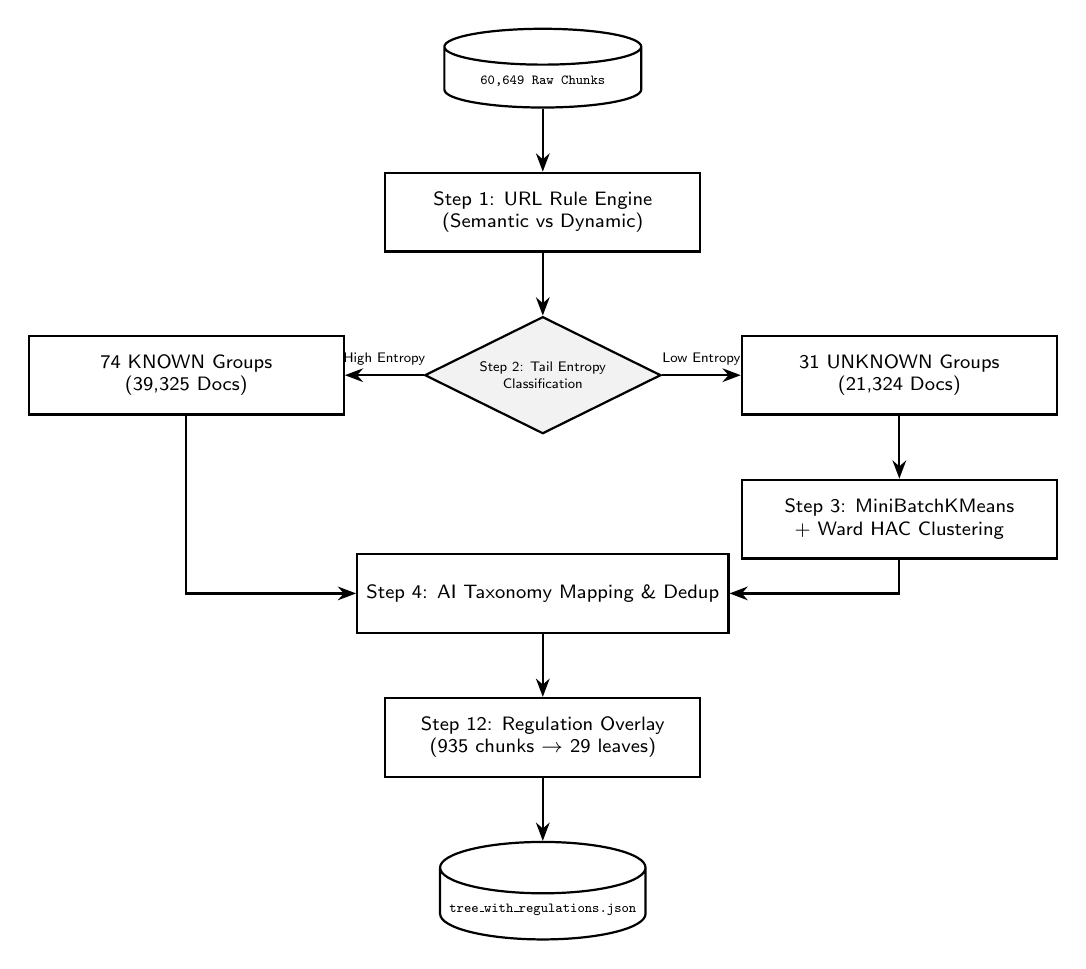
\begin{tikzpicture}[
        >=Stealth,
        node distance=1cm and 1cm,
        process/.style={rectangle, draw=black, thick, fill=white, minimum width=4cm, minimum height=1cm, align=center, font=\sffamily\scriptsize},
        decision/.style={diamond, draw=black, thick, fill=gray!10, aspect=2, minimum width=3cm, align=center, font=\sffamily\tiny},
        db/.style={cylinder, draw=black, thick, shape border rotate=90, aspect=0.25, fill=white, minimum width=2.5cm, minimum height=1cm, align=center, font=\ttfamily\tiny},
        arrow/.style={->, thick, draw=black}
    ]

    \node[db] (kb) {60,649 Raw Chunks};
    \node[process, below=0.8cm of kb] (step1) {Step 1: URL Rule Engine\\(Semantic vs Dynamic)};
    \node[decision, below=0.8cm of step1] (step2) {Step 2: Tail Entropy\\Classification};
    
    \node[process, left=1cm of step2] (known) {74 KNOWN Groups\\(39,325 Docs)};
    \node[process, right=1cm of step2] (unknown) {31 UNKNOWN Groups\\(21,324 Docs)};
    
    \node[process, below=0.8cm of unknown] (step3) {Step 3: MiniBatchKMeans\\+ Ward HAC Clustering};
    
    \node[process, below=1.5cm of step2] (step4) {Step 4: AI Taxonomy Mapping \& Dedup};
    \node[process, below=0.8cm of step4] (step12) {Step 12: Regulation Overlay\\(935 chunks $\rightarrow$ 29 leaves)};
    \node[db, below=0.8cm of step12] (final) {tree\_with\_regulations.json};

    \draw[arrow] (kb) -- (step1);
    \draw[arrow] (step1) -- (step2);
    \draw[arrow] (step2) -- node[above, font=\sffamily\tiny] {High Entropy} (known);
    \draw[arrow] (step2) -- node[above, font=\sffamily\tiny] {Low Entropy} (unknown);
    \draw[arrow] (unknown) -- (step3);
    \draw[arrow] (known) |- (step4);
    \draw[arrow] (step3) |- (step4);
    \draw[arrow] (step4) -- (step12);
    \draw[arrow] (step12) -- (final);

    \end{tikzpicture}
    }
    \caption{Data Categorization and Taxonomy Pipeline Architecture}
    \label{fig:taxonomy_pipeline}
\end{figure}

\subsection{The Orchestrator-Led Event Pipeline}
Unlike decentralized multi-agent systems, Orbis utilizes a centralized \texttt{EventPipelineOrchestrator}. This stateful hub controls stateless worker agents (\texttt{SearchAgent}, \texttt{ReasoningAgent}, \texttt{EventCreator}) to ensure database consistency and pipeline idempotency.

Figure~\ref{fig:event_system_architecture} summarizes the proactive event pipeline. The system, led by a central orchestrator, leverages specialized agents to locate sources, extract candidates, validate them, and finally store the parsed, unambiguous rules into the database while maintaining rigorous execution states.

\begin{figure}[H]
    \centering
    \resizebox{0.98\textwidth}{!}{%
    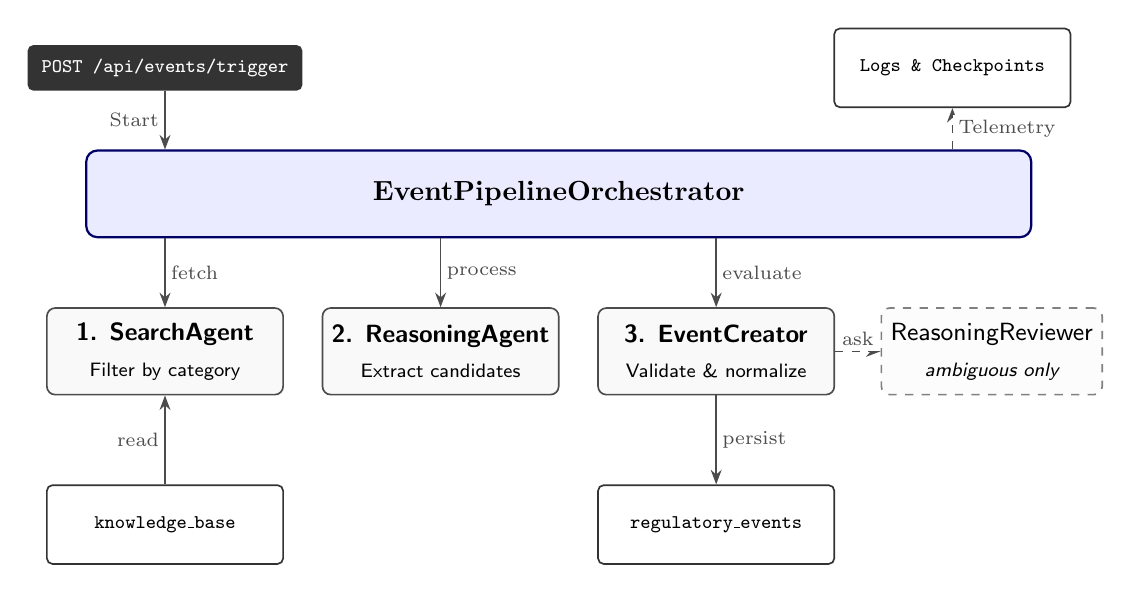
\begin{tikzpicture}[
        >=Stealth,
        font=\sffamily\small,
        node distance=1.1cm and 0.9cm,
        hub/.style={rectangle, draw=blue!40!black, line width=0.8pt, fill=blue!8,
                    rounded corners=4pt, minimum width=12cm, minimum height=1.1cm,
                    align=center, font=\bfseries},
        worker/.style={rectangle, draw=black!70, line width=0.6pt, fill=gray!5,
                       rounded corners=3pt, minimum width=3.0cm, minimum height=1.1cm,
                       align=center},
        opt/.style={rectangle, draw=black!50, line width=0.6pt, fill=gray!2, dashed,
                    rounded corners=3pt, minimum width=2.8cm, minimum height=1.1cm,
                    align=center},
        db/.style={rectangle, draw=black!80, line width=0.6pt, fill=white,
                   rounded corners=2pt, minimum width=3.0cm, minimum height=1.0cm,
                   align=center, font=\ttfamily\scriptsize},
        api/.style={rectangle, fill=black!80, text=white, rounded corners=2pt,
                    inner sep=5pt, font=\ttfamily\bfseries\scriptsize},
        lbl/.style={font=\scriptsize, text=black!70, fill=white, inner sep=2pt,
                    align=center},
        arr/.style={->, draw=black!70, line width=0.5pt},
        arrd/.style={->, draw=black!70, line width=0.5pt, dashed}
    ]

    % API trigger and telemetry sink at top
    \node[api] (trigger) at (-5,2.6) {POST /api/events/trigger};
    \node[db]  (state)   at ( 5,2.6) {Logs \& Checkpoints};

    % Central orchestrator
    \node[hub] (orch) at (0,1.0) {EventPipelineOrchestrator};

    % Worker row
    \node[worker] (search)  at (-5,-1.0) {\textbf{1. SearchAgent}\\[2pt]\scriptsize Filter by category};
    \node[worker] (reason)  at (-1.5,-1.0) {\textbf{2. ReasoningAgent}\\[2pt]\scriptsize Extract candidates};
    \node[worker] (creator) at (2.0,-1.0) {\textbf{3. EventCreator}\\[2pt]\scriptsize Validate \& normalize};
    \node[opt]    (review)  at (5.5,-1.0) {ReasoningReviewer\\[2pt]\scriptsize \itshape ambiguous only};

    % Databases at bottom
    \node[db] (kb)     at (-5,-3.2) {knowledge\_base};
    \node[db] (events) at ( 2,-3.2) {regulatory\_events};

    % Trigger -> orchestrator -> telemetry
    \draw[arr]  (trigger.south) -- (trigger.south |- orch.north) node[midway,left,lbl]{Start};
    \draw[arrd] (orch.north -| state.south) -- (state.south)     node[midway,right,lbl]{Telemetry};

    % Orchestrator -> workers
    \draw[arr] (orch.south -| search.north)  -- (search.north)  node[midway,right,lbl]{fetch};
    \draw[arr] (orch.south -| reason.north)  -- (reason.north)  node[midway,right,lbl]{process};
    \draw[arr] (orch.south -| creator.north) -- (creator.north) node[midway,right,lbl]{evaluate};

    % Workers -> DBs
    \draw[arr] (kb.north)      -- (search.south)  node[midway,left,lbl]{read};
    \draw[arr] (creator.south) -- (events.north)  node[midway,right,lbl]{persist};

    % Optional reviewer
    \draw[arrd] (creator.east) -- (review.west) node[midway,above,lbl]{ask};

    \end{tikzpicture}}
    \caption{Sequential flow and architecture of the Orbis Proactive Event Pipeline. The orchestrator owns all run state; workers are stateless and communicate only via the orchestrator. The reviewer is invoked only for ambiguous candidates.}
    \label{fig:event_system_architecture}
\end{figure}

To prevent non-actionable events from reaching students, extraction follows a \textbf{Two-Pass LLM Adversarial Review}:
\begin{enumerate}
    \item \textbf{Pass 1 (Extraction):} The model evaluates full documents to generate candidate rules, defining triggers, deadlines, and target roles.
    \item \textbf{Pass 2 (Adversarial Fix):} The model reviews the original document alongside Pass 1 output to actively remove stale items, fix weak wording, and add missed rules.
\end{enumerate}

\subsection{Contextual vs. SQL Assignment Matching}
User assignments are routed through two parallel channels based on the user's \texttt{extra\_context} JSON profile:
\begin{itemize}
    \item \textbf{SQL Path (Deterministic):} Objective thresholds (e.g., GPA constraints) are evaluated instantly via Python logic against database variables.
    \item \textbf{Contextual Path (LLM Reasoned):} Complex rules are evaluated against the student's text profile in batches. The LLM determines applicability and generates a human-readable justification.
\end{itemize}

\subsection{Agentic Assignment Submission Evaluation}
Beyond proactively assigning obligations, Orbis also evaluates work students submit against those assignments. Each upload is processed by a stateless \texttt{submission\_agent} that, rather than issuing a single opaque verdict, reasons in causal steps that mirror how a human teaching assistant screens a submission: first understand \emph{what is being asked}, then check the document \emph{against each individual requirement} with cited evidence, and only then decide. Concretely the agent runs a deterministic file gate followed by a two-call LLM reasoning chain.

\begin{enumerate}
    \item \textbf{File inspection (no LLM).} The agent records the file's extension, size, MIME type, and --- for archives --- the member list. Empty files, oversized files, archives over a configured member limit, and unreadable or unsupported payloads are rejected here without ever invoking the LLM.
    \item \textbf{Text extraction.} Supported formats (\texttt{.pdf}, \texttt{.docx}, \texttt{.zip}, and ${\sim}70$ text-like extensions) are decoded to plain text. Inside archives the agent no longer trusts the extension as a gate: it skips only known-binary types and otherwise attempts to decode each member, keeping it if a printable-character heuristic confirms it is text (so a \texttt{.tex} project or an extensionless \texttt{Makefile} is still read).
    \item \textbf{Requirement decomposition (LLM call 1).} The agent prompts the LLM to break the assignment title and description into a checklist of discrete, independently checkable requirements. If this call yields nothing usable, the agent falls back to a deterministic keyword \texttt{line\_review} derived from the assignment text so the next step always has structure to anchor on.
    \item \textbf{Per-requirement judgment and decision (LLM call 2).} The agent prompts the LLM with the requirement checklist, the file profile, and the extracted text (clipped to a configured budget), and asks it to walk \emph{each} requirement: does the document satisfy it, with a quoted evidence span and a causal justification of \emph{why}. Only after every requirement is judged does the model synthesize the overall \texttt{approved}/\texttt{rejected} decision. The output is a structured JSON report containing a \texttt{requirement\_findings} array (one \{satisfied, evidence, evidence\_line, reasoning\} object per requirement) plus a confidence score and a student-facing reason.
\end{enumerate}

The entire flow is exposed to the browser as a Server-Sent-Events stream: the client receives the extracted source text, the decomposed requirements, and each per-requirement finding as it is produced, and renders them live alongside a chronological ``agent work'' trail and a source-document panel that highlights the exact passage each finding references. If the agent rejects the submission, the student is presented with the reason and a \texttt{flag\_for\_review} action that records \texttt{flagged\_by\_student} and \texttt{student\_flag\_reason} on the submission row and routes the case to a human reviewer. This appeal path is, in our view, an ethical requirement: it prevents an automated false rejection from terminating a student's chance to be graded.

\begin{figure}[H]
    \centering
    \resizebox{0.96\textwidth}{!}{%
    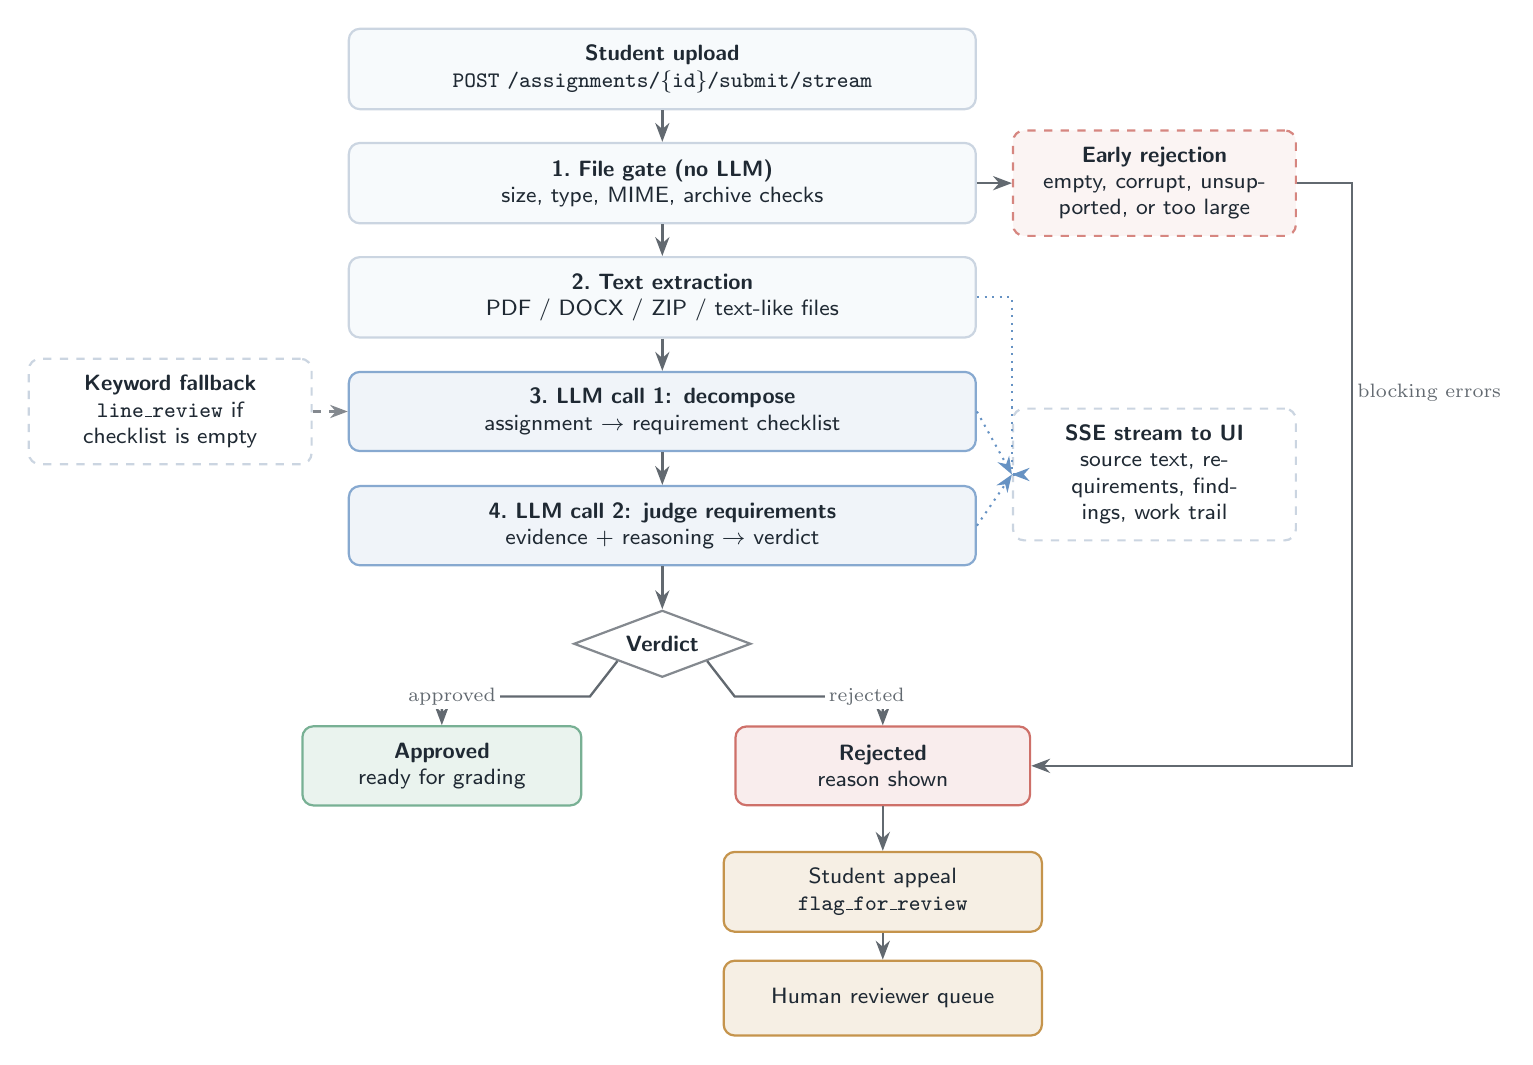
\begin{tikzpicture}[
        x=1cm,
        y=1cm,
        >=Stealth,
        font=\sffamily\footnotesize,
        block/.style={rectangle, draw=orbisLine, line width=0.8pt, fill=white,
                      rounded corners=4pt, align=center, text=orbisInk,
                      inner xsep=8pt, inner ysep=6pt, text width=7.4cm,
                      minimum height=0.9cm},
        stage/.style={block, fill=orbisPanel},
        llmstage/.style={block, draw=orbisBlue!55, fill=orbisBlue!7},
        aux/.style={rectangle, draw=orbisLine, dashed, line width=0.8pt,
                    fill=white, rounded corners=4pt, align=center,
                    text=orbisInk, inner xsep=7pt, inner ysep=6pt, text width=3.1cm,
                    minimum height=0.95cm},
        rejectaux/.style={aux, draw=orbisRed!55, fill=orbisRed!5},
        decision/.style={diamond, aspect=2.25, draw=orbisInk!55, line width=0.8pt,
                         fill=white, align=center, text=orbisInk,
                         inner sep=1pt, minimum width=2.25cm, minimum height=0.85cm},
        ok/.style={rectangle, draw=orbisGreen!65, line width=0.8pt,
                   fill=orbisGreen!10, rounded corners=4pt, align=center,
                   text=orbisInk, inner xsep=7pt, inner ysep=6pt,
                   text width=3.05cm, minimum height=1.0cm},
        bad/.style={rectangle, draw=orbisRed!65, line width=0.8pt,
                    fill=orbisRed!8, rounded corners=4pt, align=center,
                    text=orbisInk, inner xsep=7pt, inner ysep=6pt,
                    text width=3.25cm, minimum height=1.0cm},
        human/.style={rectangle, draw=orbisGold!80, line width=0.8pt,
                      fill=orbisGold!12, rounded corners=4pt, align=center,
                      text=orbisInk, inner xsep=7pt, inner ysep=6pt,
                      text width=3.55cm, minimum height=0.95cm},
        arrow/.style={->, draw=orbisInk!70, line width=0.85pt},
        softarrow/.style={->, draw=orbisBlue!70, dotted, line width=0.75pt},
        fallback/.style={->, draw=orbisInk!55, dashed, line width=0.75pt},
        lbl/.style={font=\scriptsize, text=orbisInk!70, fill=white, inner sep=1.5pt}
    ]

    % Main submission pipeline
    \node[stage]    (upload)  at (0,  7.50) {\textbf{Student upload}\\ \texttt{POST /assignments/\{id\}/submit/stream}};
    \node[stage]    (inspect) at (0,  6.05) {\textbf{1.~File gate (no LLM)}\\ size, type, MIME, archive checks};
    \node[stage]    (extract) at (0,  4.60) {\textbf{2.~Text extraction}\\ PDF / DOCX / ZIP / text-like files};
    \node[llmstage] (decomp)  at (0,  3.15) {\textbf{3.~LLM call 1: decompose}\\ assignment $\rightarrow$ requirement checklist};
    \node[llmstage] (judge)   at (0,  1.70) {\textbf{4.~LLM call 2: judge requirements}\\ evidence + reasoning $\rightarrow$ verdict};
    \node[decision] (verdict) at (0,  0.20) {\textbf{Verdict}};

    % Side lanes
    \node[rejectaux] (early) at (6.25, 6.05) {\textbf{Early rejection}\\ empty, corrupt, unsupported, or too large};
    \node[aux] (kw) at (-6.25, 3.15) {\textbf{Keyword fallback}\\ \texttt{line\_review} if checklist is empty};
    \node[aux] (sse) at (6.25, 2.35) {\textbf{SSE stream to UI}\\ source text, requirements, findings, work trail};

    % Outcomes
    \node[ok]    (approve) at (-2.8, -1.35) {\textbf{Approved}\\ ready for grading};
    \node[bad]   (reject)  at ( 2.8, -1.35) {\textbf{Rejected}\\ reason shown};
    \node[human] (flag)    at ( 2.8, -2.95) {Student appeal\\ \texttt{flag\_for\_review}};
    \node[human] (queue)   at ( 2.8, -4.30) {Human reviewer queue};

    % Primary path
    \draw[arrow] (upload) -- (inspect);
    \draw[arrow] (inspect) -- (extract);
    \draw[arrow] (extract) -- (decomp);
    \draw[arrow] (decomp) -- (judge);
    \draw[arrow] (judge) -- (verdict);
    \draw[arrow] (verdict.south west) -- ++(-0.35,-0.45) -| (approve.north)
        node[pos=0.30,left,lbl]{approved};
    \draw[arrow] (verdict.south east) -- ++(0.35,-0.45) -| (reject.north)
        node[pos=0.30,right,lbl]{rejected};

    % Exceptions, fallback, and live UI stream
    \draw[arrow] (inspect.east) -- (early.west);
    \draw[arrow] (early.east) -- ++(0.70,0) |- (reject.east)
        node[pos=0.18,right,lbl]{blocking errors};
    \draw[fallback] (kw.east) -- (decomp.west);
    \draw[softarrow] (extract.east) -- ++(0.45,0) |- (sse.west);
    \draw[softarrow] (decomp.east) -- (sse.west);
    \draw[softarrow] (judge.east) -- (sse.west);

    % Appeal path
    \draw[arrow] (reject) -- (flag);
    \draw[arrow] (flag) -- (queue);

    \end{tikzpicture}}
    \caption{Agentic submission-evaluation flow. A deterministic file gate rejects empty, corrupt, or unreadable files without invoking the LLM. The agent then reasons in two LLM calls: it first \emph{decomposes} the assignment into a requirement checklist, then \emph{judges the document against each requirement individually} with cited evidence before synthesizing a verdict. A deterministic keyword \texttt{line\_review} is retained only as a fallback when decomposition fails. Every stage is streamed over Server-Sent Events so the UI can render the source text, the requirements, and each per-requirement finding live. Every rejection (early-stage or LLM-based) is recoverable through the \texttt{flag\_for\_review} appeal path, which routes the case to a human reviewer instead of terminating the student's submission attempt.}
    \label{fig:submission_flow}
\end{figure}

\subsection{RAG Chatbot Architecture}
\label{sec:rag_arch}

The Orbis RAG chatbot is a stateless, multi-agent pipeline for answering natural-language queries over the institutional knowledge base. Its design prioritizes \textit{precision} and \textit{fault tolerance} over conversational continuity: no conversation history is retained between queries, preventing context bloat and token overflow while ensuring each query receives the full retrieval budget. Figure~\ref{fig:rag_flow} illustrates the end-to-end query flow.

\begin{figure}[H]
    \centering
    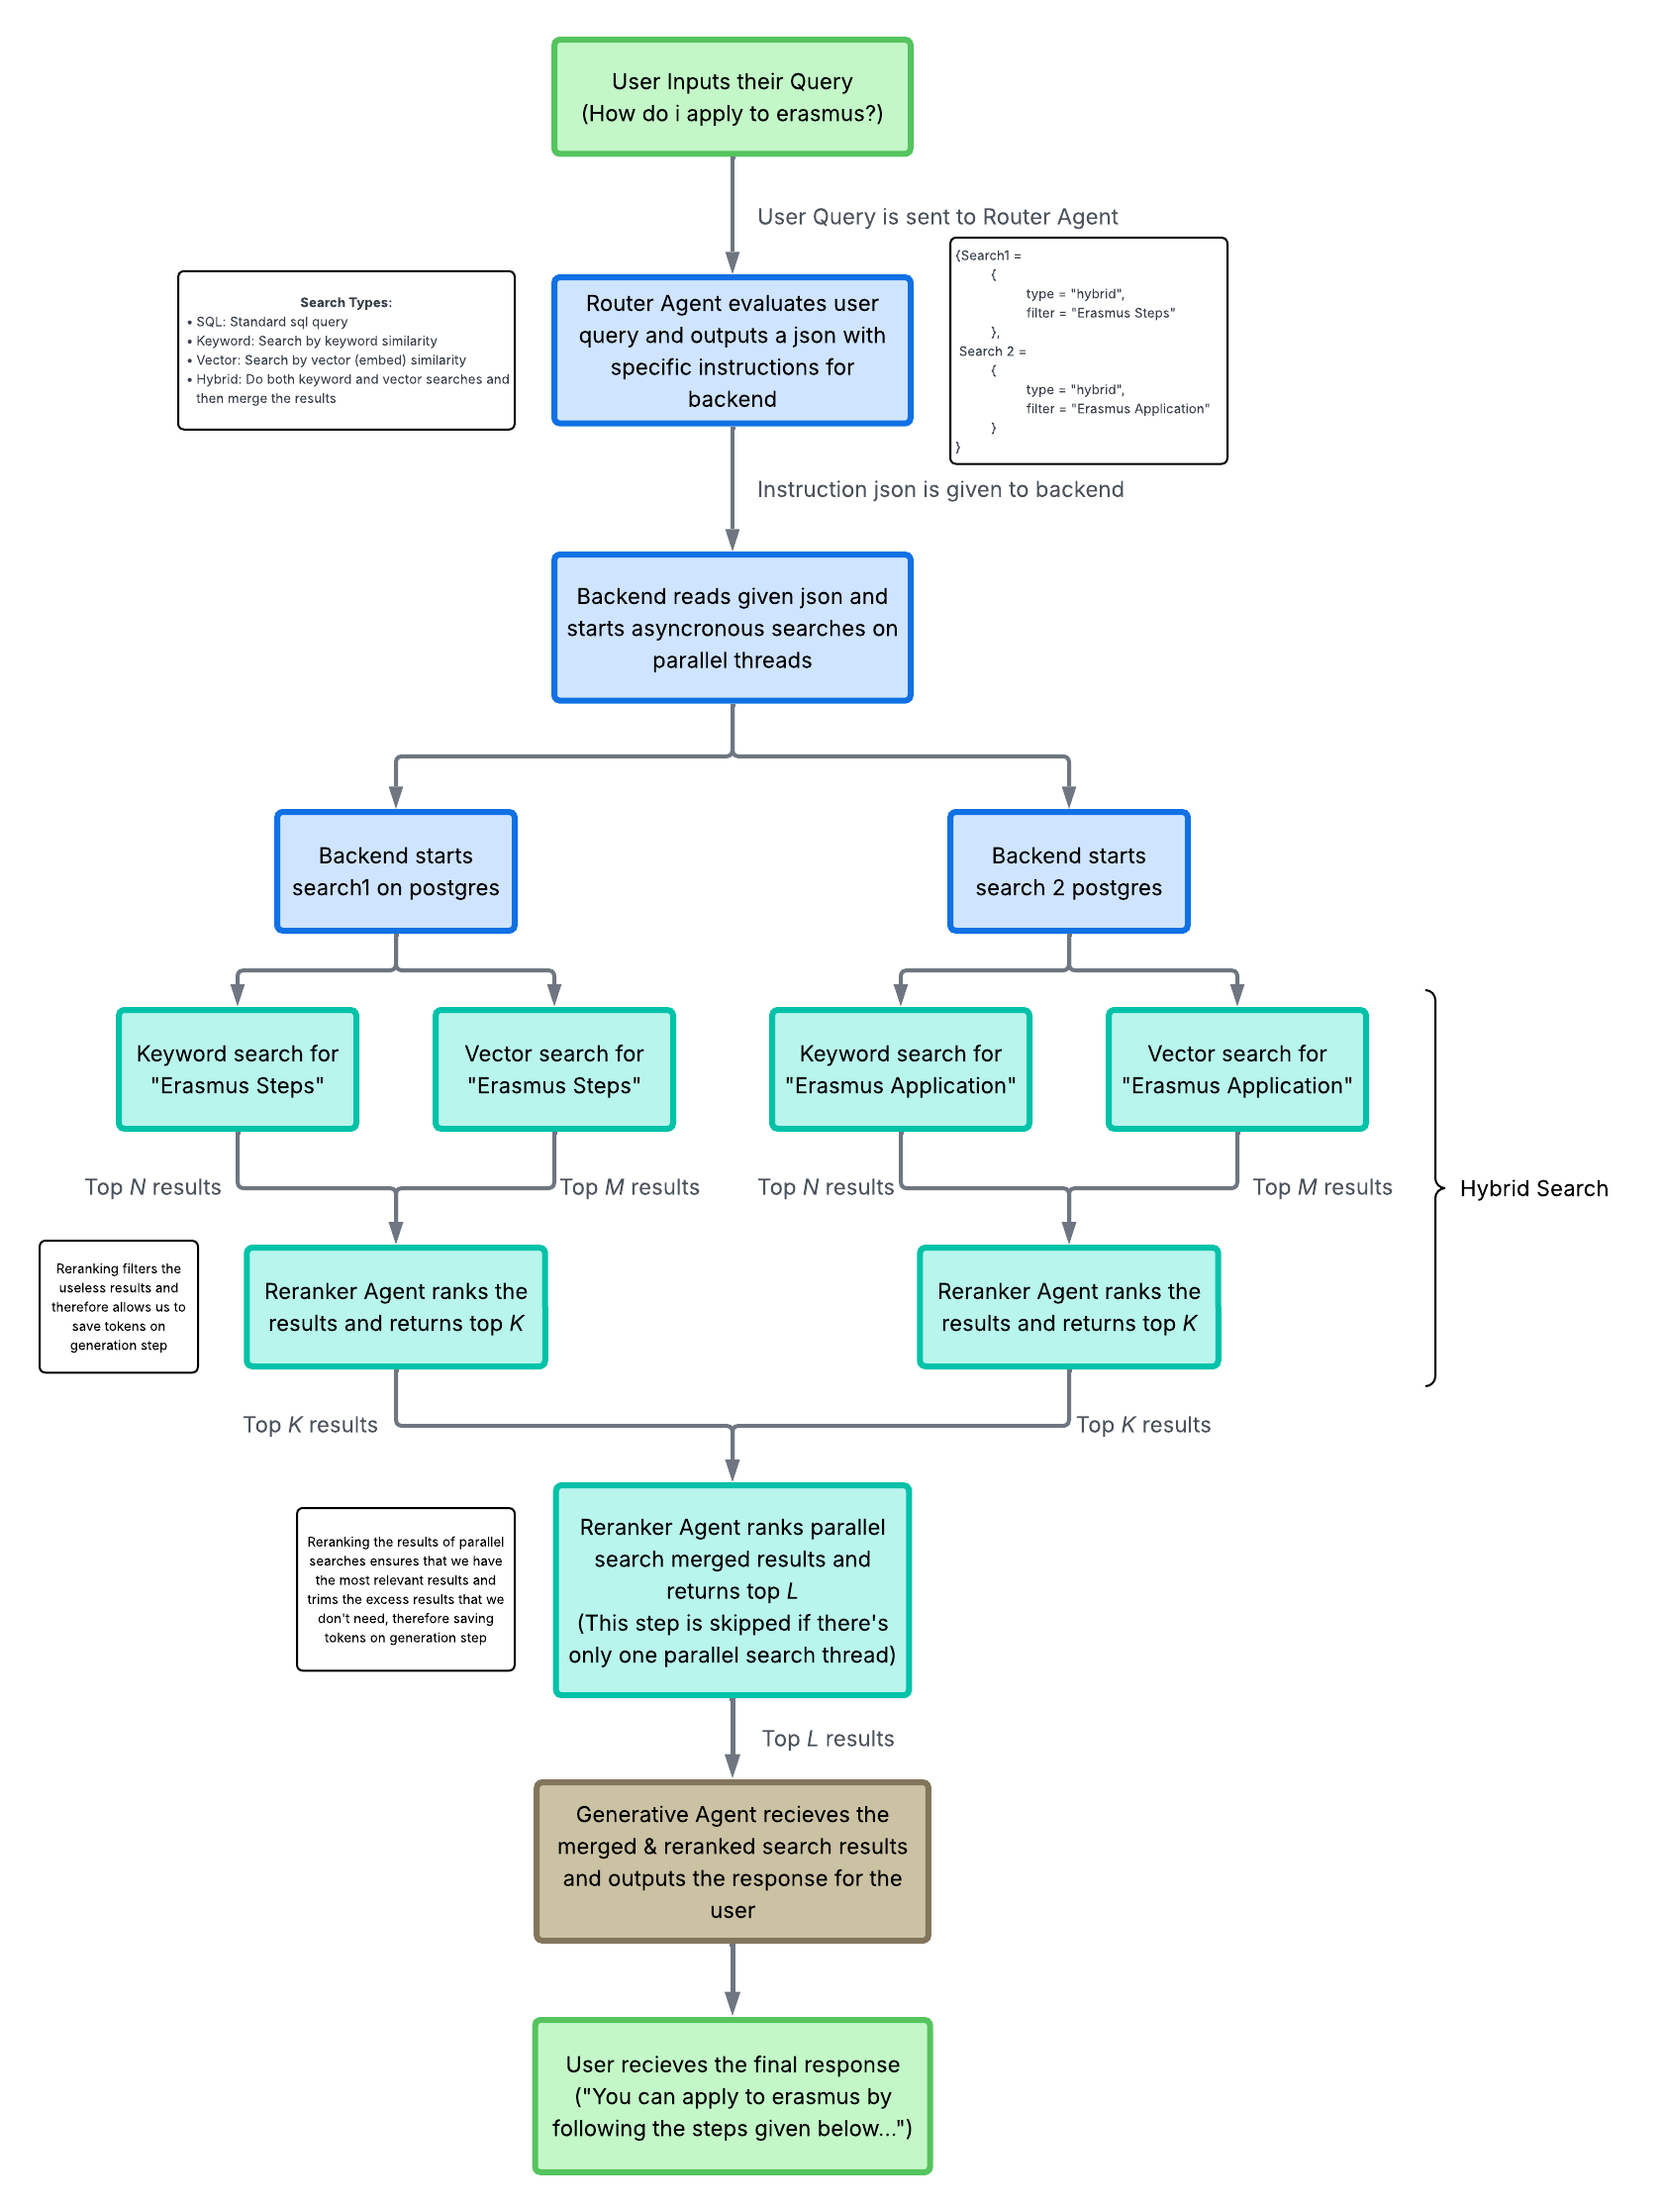
\includegraphics[width=0.95\textwidth]{figures/Orbis_RAG_General_Flow_Diagram.png}
    \caption{End-to-end RAG chatbot pipeline. The Router Agent converts the user query to a structured intent list; the backend dispatches parallel hybrid searches; each search undergoes Reranker-scored ranking before results are merged, optionally re-ranked across intents, and passed to the Generative Agent for a streamed final response.}
    \label{fig:rag_flow}
\end{figure}

\subsubsection{Knowledge Base Construction and Ingestion Pipeline}

The data pipeline that populates the \texttt{knowledge\_base} table runs in three sequential steps. First, \texttt{fix\_pdf\_language\_and\_titles.py} sanitizes PDF metadata using the stopword race language detector described in Section~3.1. Second, \texttt{load\_data.py} reads the JSONL source files, splits web page and PDF content into \textbf{150-word chunks with 30-word overlap} (hard-capped to stay within the embedding model's context limit), and inserts records with \texttt{embedding = NULL}. Separating ingestion from embedding keeps the bulk load fast. Third, \texttt{embed\_database.py} generates 384-dimensional vectors for all null-embedding rows in configurable batch sizes.

A critical detail is the \textit{enriched embedding format}: before vectorization, each document's title and categorical context are prepended to the content. For web pages, the full breadcrumb path is prepended (e.g., \texttt{BİLGİ'de Yaşam > Ulaşım > Servis > Güzergah}); for courses, the course code is prepended. This ensures the embedding model encodes both the content topic and its institutional category in a single vector, improving retrieval specificity for navigation-structured content.

The selected embedding model, \texttt{sentence-transformers/paraphrase-multilingual-MiniLM-L12-v2}, produces 384-dimensional vectors and natively handles both Turkish and English. The model is served via a Text Embeddings Inference (TEI) container with a local in-process Hugging Face fallback. Two PostgreSQL indexes are maintained: an HNSW index on the \texttt{embedding} column (L2 distance) for approximate nearest-neighbor vector search, and a GIN index on the auto-generated \texttt{search\_vector} TSVECTOR column for full-text keyword search.

\subsubsection{LLM-Based Query Routing}

Every query is first processed by a \textbf{Router Agent} (an LLM call via Groq \texttt{llama-3.3-70b-versatile}) prompted to output a structured JSON ``intent list'' directing the retrieval engine. Four tools are available:

\begin{itemize}
    \item \textbf{\texttt{sql}:} Specific course code or department list queries. Carries SQL filter fields (\texttt{code}, \texttt{title\_like}).
    \item \textbf{\texttt{vector}:} All semantic, regulatory, and procedural queries. Default for anything not covered by the three SIS tools.
    \item \textbf{\texttt{calendar}:} Academic date queries (e.g., ``When are midterms?''). Triggers a lookup in the SIS \texttt{academic\_calendar\_entries} table.
    \item \textbf{\texttt{student\_schedule}:} Personal timetable queries (e.g., ``What are my classes today?''). Triggers a lookup of the authenticated user's enrolled sections.
\end{itemize}

Multi-intent queries (comparing two courses, or spanning a regulation and a calendar date) return multiple intents. Each is executed in parallel with a reduced per-intent budget (\texttt{TOP\_K=15}, \texttt{FINAL\_K=5}) to conserve the context window across the merged result. Router output is auto-repaired: a \texttt{sql} intent with no filters falls back to \texttt{vector}; malformed JSON produces a single \texttt{vector} intent from the raw query string.

Calendar and schedule intents are intercepted before the retrieval engine by \texttt{context\_injectors.py}, which fetches structured data from the SIS relational tables and formats it as a structured \texttt{AKADEMİK TAKVİM} (academic calendar) or \texttt{ÖĞRENCİ HAFTALIK PROGRAMI} (personal schedule) block. This block is prepended to the RAG document context before generation, allowing the LLM to reason over both structured SIS data and unstructured document chunks in a single prompt. Both fetchers are wrapped in try/except so SIS failures do not interrupt the retrieval pipeline.

\subsubsection{Hybrid Search with Two-Stage Neural Re-Ranking}

For each \texttt{vector} intent the pipeline executes four stages:

\begin{enumerate}
    \item \textbf{Hybrid Search.} \texttt{rag\_repository.vector\_search()} executes a TSVector keyword query and an HNSW vector similarity search concurrently. Results merge with keyword matches \textit{first} (higher precision), then vector matches (higher semantic recall), with de-duplication by document ID. The combined pool contains up to \texttt{TOP\_K=30} candidates.

    \item \textbf{Pre-Expansion Rerank.} The full 30-candidate pool is submitted to the Jina AI cross-encoder reranker, which identifies the ``True Top 3'' most relevant source documents. This quality filter runs \textit{before} expansion. Without it, the expansion step would reconstruct full documents from irrelevant sources, flooding the context window.

    \item \textbf{Smart Context Expansion.} For each of the True Top 3 documents (\texttt{type=web\_page} or \texttt{type=pdf}), all chunks sharing the same source URL are fetched via \texttt{rag\_repository.get\_by\_url()}. This reconstructs the complete source document around the highest-ranked retrieval hits, bypassing the 150-word chunk limit for multi-article regulatory texts. A regulation spanning 5--10 chunks is presented in full rather than as an isolated fragment. The expansion pool is capped at 75 candidates.

    \item \textbf{Final Rerank.} The expanded pool is re-submitted to the Jina AI reranker. This stage selects the \texttt{FINAL\_K=10} chunks most relevant within the reconstructed documentary context for delivery to the LLM.
\end{enumerate}

The two-stage architecture is the most critical design decision in the pipeline. A single reranking pass applied after expansion faces a candidate pool dominated by irrelevant neighboring chunks, which suppresses genuinely relevant documents. The pre-expansion pass preserves the quality signal; the post-expansion pass maximizes contextual completeness.

\subsubsection{Context Building and Streaming Response Generation}

After deduplication across all intents, \texttt{context.py} assembles the final prompt. For SQL results returning more than 5 items, or when the total candidate set exceeds 40 documents, a \textbf{CSV Compacting} mode condenses the data to a tabular format containing only essential fields (e.g., course codes and ECTS values), preventing context window overflow. For normal retrieval, each document is rendered as a detailed text block (title, URL, breadcrumb metadata, content).

The compiled context---including any prepended SIS blocks---is passed to the generative LLM with a system prompt enforcing four rules: (1) Markdown citation links on document titles, never on entity names; (2) no fabricated citations; (3) when an answer involves a procedure, the responsible office must be named and contact advised; (4) structured SIS blocks are authoritative, non-citable data. The LLM response streams back via Server-Sent Events (SSE) for immediate token-by-token display.

\section{Experimental Setup}
\subsection{Framework and Deployment}
The backend is implemented in Python 3.10 with the FastAPI framework and served by Uvicorn. Persistent storage is provided by PostgreSQL extended with the \texttt{pgvector} extension; the same database stores both the relational schema (users, courses, rules, assignments, telemetry) and the embedding index. The application runtime supports Gemini, Groq, and OpenAI-compatible LLM providers through environment configuration, while the evaluation scripts used for this report route judge calls through OpenRouter so that model choice and cost are explicit. For the experiments reported in Section~9, the bulk LLM workload (labeling, extraction review, submission reasoning) uses \texttt{google/gemini-2.5-flash-lite}, with \texttt{deepseek/deepseek-v3.2} reserved for the adversarial Pass~2 review and \texttt{qwen/qwen3-235b-a22b-2507} used as the secondary judge during cross-validation. Document embeddings are produced offline by a local MiniLM model and reused at query time; the repository also includes an optional Docker Compose setup that load-balances TEI embedding servers behind Nginx.

The quantitative regulation-assignment results should be read as an evaluation of the preserved action-object pipeline artifacts in the project database: \texttt{regulation\_rules}, \texttt{user\_rule\_assignments}, and \texttt{event\_candidate\_logs}. The current repository also contains a newer admin-triggered extraction route that writes accepted rows to \texttt{regulatory\_events}. This implementation boundary does not change the reported metrics, but it clarifies that the assignment-matching evaluation is tied to the archived database run rather than to a live, currently exposed \texttt{/api/events/assign/me} endpoint.

\subsection{Performance Metrics}
The system's rule extraction efficacy is evaluated fundamentally on its \textit{Acceptance Rate} and qualitative precision. A successful pipeline must maximize true positive obligations while forcefully rejecting noisy, non-imperative fragments.
$$Accuracy = \frac{TP + TN}{TP + TN + FP + FN}$$
$$Precision = \frac{TP}{TP + FP}$$
$$Recall = \frac{TP}{TP + FN}$$
$$F_1 = 2 \cdot \frac{Precision \cdot Recall}{Precision + Recall}$$

\subsection{RAG Chatbot System Configuration}

The RAG chatbot is exposed via the \texttt{/api/chat} endpoint of the same FastAPI application. Key retrieval parameters are: \texttt{RAG\_TOP\_K=30} (initial hybrid pool size), \texttt{RAG\_FINAL\_K=10} (documents passed to the LLM after final re-ranking), and \texttt{EMBEDDING\_DIM=384}. The embedding service is provider-agnostic: \texttt{tei} (locally hosted TEI container), \texttt{ollama}, or \texttt{local} (in-process Hugging Face model). Re-ranking uses the Jina AI API (\texttt{jina-reranker-v2-base-multilingual}) with an index-order fallback. The LLM generation layer supports Groq (\texttt{llama-3.3-70b-versatile}) and Google Gemini (\texttt{gemini-1.5-flash}) via a common streaming wrapper selectable at runtime.

\subsection{RAG Evaluation Dataset}

The RAG pipeline was evaluated against a standardized benchmark of \textbf{100 bilingual (Turkish and English) queries} derived from actual Bilgi University data present in the knowledge base. The benchmark is designed to cover every routing tool and every architectural feature of the pipeline. Table~\ref{tab:rag_eval_dataset} summarizes the seven query categories.

\begin{table}[H]
    \centering
    \begin{adjustbox}{center}
        \begin{tabular}{l c c l}
            \toprule
            \textbf{Category} & \textbf{Query IDs} & \textbf{Count} & \textbf{Feature Tested} \\ \midrule
            Direct Course Inquiries   & 001--020 & 20 & \texttt{sql} routing, exact field lookup \\
            Bulk Course Inquiries     & 021--030 & 10 & \texttt{sql} + CSV Compacting \\
            Personal Schedule         & 031--035 &  5 & \texttt{student\_schedule} SIS injection \\
            Academic Calendar         & 036--040 &  5 & \texttt{calendar} SIS injection \\
            Academic Regulations      & 041--065 & 25 & \texttt{vector} + Smart Context Expansion (PDFs) \\
            Campus Life \& Facilities & 066--085 & 20 & \texttt{vector} retrieval via web pages \\
            Multi-hop / Comparison    & 086--100 & 15 & Parallel multi-intent routing \\
            \bottomrule
        \end{tabular}
    \end{adjustbox}
    \caption{RAG evaluation benchmark: 100 bilingual queries across seven routing categories}
    \label{tab:rag_eval_dataset}
\end{table}

\subsection{RAG Evaluation Metrics}

Five metrics cover the complete query-to-answer lifecycle:
\begin{itemize}
    \item \textbf{Routing Accuracy:} Percentage of queries for which the Router Agent selected the correct tool(s) and applied correct filters, adjusted for anomalies in the ground-truth dataset (e.g., filters referencing database fields that do not exist in the production schema).
    \item \textbf{Context Recall:} Percentage of queries for which the required source data was present in the final retrieved context, regardless of routing path.
    \item \textbf{Mean Reciprocal Rank (MRR):} Ranking quality of the final reranked result set. An MRR of 1.0 indicates the relevant document is always in the top position.
    \item \textbf{Semantic Accuracy:} LLM-judged metric (consistent with the LLM-as-a-judge methodology of Section~2) assessing factual alignment between the generated answer and the retrieved context.
    \item \textbf{Answer F1-Score (Token Overlap):} Lexical measure of token-level overlap between the generated answer and the expected ground-truth answer string.
\end{itemize}

\section{Experiments \& Discussion}
The Orbis backend was rigorously evaluated using production database logs (Run ID: \texttt{fadc244f...}) to measure both extraction throughput and assignment precision. 

\subsection{Extraction Throughput \& Quality Funnel}
The complete pipeline processed 80 regulation sources in exactly 59 minutes. During this run, the Orchestrator evaluated 323 candidate rules. 

\begin{table}[H]
    \centering
    \begin{adjustbox}{center}
        \begin{tabular}{l c}
            \toprule
            \textbf{Pipeline Metric} & \textbf{Value} \\ \midrule
            Source Documents Processed & 80 \\
            KB Chunks Consumed & 935 \\
            Candidate Rules Evaluated & 323 \\
            \textbf{Accepted Active Rules} & \textbf{178 (55\%)} \\
            Rejected Quality Candidates & 145 (45\%) \\
            \bottomrule
        \end{tabular}
    \end{adjustbox}
    \caption{Event Extraction Pipeline Funnel}
    \label{tab:extraction_funnel}
\end{table}

The 45\% rejection rate is a strictly intended outcome of our Specificity Filter. Of the 145 rejected candidates, 128 were flagged precisely for being "not imperative enough," while others were rejected for "audience too broad" or "awareness only wording." This ensures students are only notified of strict, actionable obligations.

\subsection{RAG Chatbot Evaluation}
\label{sec:rag_experiments}

The 100-query bilingual benchmark was executed end-to-end against the live Orbis pipeline. A JSONL evaluation log was written at runtime for each query, capturing router output, hybrid search candidates, reranker scores, expansion decisions, and the final generated response. Table~\ref{tab:rag_results} presents the aggregate results.

\begin{table}[H]
    \centering
    \begin{adjustbox}{center}
        \begin{tabular}{l c}
            \toprule
            \textbf{Metric} & \textbf{Score} \\ \midrule
            Routing Accuracy                & $\approx$92\% \\
            Context Recall                  & $\approx$95\% \\
            Mean Reciprocal Rank (MRR)      & $\approx$0.94 \\
            Semantic Accuracy               & $\approx$98\% \\
            Answer F1-Score (Token Overlap) & $\approx$78\% \\
            \bottomrule
        \end{tabular}
    \end{adjustbox}
    \caption{RAG chatbot evaluation results on the 100-query bilingual benchmark}
    \label{tab:rag_results}
\end{table}

The primary routing failure mode was routing descriptive course questions (e.g., ``Who is the target audience for ACC 516?'') to \texttt{vector} instead of \texttt{sql}. These deviations did not degrade the final answer: the vector search successfully embedded the query and located the relevant course chunk, demonstrating the architecture's cross-path fault tolerance. Smart Context Expansion proved essential for the Regulations category (Q041--Q065): procedural questions such as ``How do I appeal a final exam grade?'' triggered expansion against the relevant PDF, delivering the complete multi-step procedure instead of a single 150-word fragment. The 78\% F1 score is intentionally lower than Semantic Accuracy: the generative model enriches raw database values with auxiliary information (source URLs, office contact advice), producing answers that are more helpful than the concise ground-truth strings but lexically divergent from them.

\section{Results}
The system's assignment logic was exercised against the 4 student profiles stored in \texttt{user\_profiles}. The pipeline produced 176 active rows in \texttt{user\_rule\_assignments}, distributed across profiles and match types as reported in Table~\ref{tab:assignment_results}.

\begin{table}[H]
    \centering
    \begin{adjustbox}{center}
        \begin{tabular}{p{6.2cm} c c c c c}
            \toprule
            \textbf{Profile (real \texttt{user\_profiles} row)} & \textbf{Total} & \textbf{High} & \textbf{Med} & \textbf{SQL} & \textbf{CTX} \\ \midrule
            P1: CSE, Year~2 Sem~3, on probation, no internship yet & 42 & 30 & 8 & 8 & 34 \\
            P2: Business Admin, Year~3 Sem~5, double major, merit scholarship & 36 & 25 & 6 & 3 & 33 \\
            P3: CSE, Year~4 Sem~7, graduation project in progress & 60 & 38 & 17 & 2 & 58 \\
            P4: CSE, Year~3 Sem~6, mandatory internship required, no company yet & 38 & 29 & 5 & 2 & 36 \\
            \bottomrule
        \end{tabular}
    \end{adjustbox}
    \caption{Assignments generated per real student profile, broken down by urgency and matching path. ``SQL'' counts deterministic conditional matches; ``CTX'' counts contextual LLM matches.}
    \label{tab:assignment_results}
\end{table}

The contextual path produced specific, situation-aware assignments. For profile P4 (CSE Y3, mandatory internship required, no company yet, internship form not submitted), the matcher surfaced internship-specific obligations such as \emph{``Submit the Internship Contract Cover Form at least 10 working days before your start date,''} explicitly because the \texttt{internship\_form\_submitted} flag was false. The deterministic SQL path complemented this for objective, threshold-style rules: profile P1 (on probation) triggered 8 SQL-matched rules tied to GPA-conditional regulations, bypassing the LLM entirely and reducing latency and cost on rules that do not require contextual reasoning.

We re-emphasize that the figures above describe \emph{coverage}, not \emph{correctness}: how many assignments were emitted, not how many were right. The corresponding correctness analysis is presented in Section~9.3.

\section{Quantitative Evaluation}
While the aggregate counts in Tables~\ref{tab:extraction_funnel} and~\ref{tab:assignment_results} describe the system's throughput, they do not assess whether each individual decision was \emph{correct}. To answer that question we constructed a labeled evaluation set and report per-stage precision, recall, $F_1$, and a stratum-level error analysis. 

The interpretation of these metrics follows the comparator boundaries established in Table~\ref{tab:baseline_validity}. The only direct baseline claim in this report is internal: the current two-call submission reviewer improves over the prior Orbis single-call reviewer on the same case design. External official works are used more cautiously. The event-extraction precision can be discussed alongside regulatory IE systems such as Zhang and El-Gohary or Galli et al., but it is not a direct win/loss claim because the source domain and output schema differ. Assignment matching has no exact official baseline found in the literature; submission review is also not directly comparable to JorGPT because Orbis performs binary accept/reject screening with appeal rather than numerical grade regression.

\subsection{Gold Ground-Truth Construction}
To rigorously evaluate the system, human domain experts (the authors) manually annotated all 323 extraction candidates and 712 profile-obligation pairs to establish a Gold Ground Truth. 

For the submission agent, ground truth was generated deterministically by constructing 8 strata over each of the 4 real assignments in the database (32 cases total): \texttt{approve}, \texttt{approve\_multifile}, \texttt{reject\_wrong\_content} (a file from a different assignment), \texttt{reject\_empty}, \texttt{reject\_corrupt} (random bytes in a PDF wrapper), \texttt{reject\_wrong\_ext} (Python source renamed to \texttt{.pdf}), \texttt{flag\_partial} (LLM-written incomplete draft), and \texttt{reject\_injection} (wrong-content document appended with a prompt-injection payload instructing the reviewer to approve). Each case contains a requirement file, a directory of submitted files, and an \texttt{expected.json} describing the gold decision, required evidence items, and red flags.

Table~\ref{tab:metric_provenance} lists the provenance of every quantitative claim used in the evaluation. This table is intentionally included to make the evidence boundary explicit: the event and assignment labels are human-validated gold labels, while the submission cases have deterministic expected labels but are small and synthetic.

\begin{table}[H]
\centering
\scriptsize
\begin{adjustbox}{width=\textwidth}
\setlength{\tabcolsep}{3pt}
\begin{tabular}{>{\raggedright\arraybackslash}p{3.0cm}>{\raggedright\arraybackslash}p{2.2cm}>{\raggedright\arraybackslash}p{3.3cm}>{\raggedright\arraybackslash}p{3.6cm}>{\raggedright\arraybackslash}p{4.4cm}}
\toprule
\textbf{Metric family} & \textbf{Reported value} & \textbf{Evaluation set} & \textbf{Artifact or script} & \textbf{Limitation} \\ \midrule
Event extraction & Precision 0.978; recall 0.574; $F_1$ 0.723 & 323 candidates from \texttt{event\_candidate\_logs} & \texttt{events/}\newline \texttt{candidates\_gt.jsonl}\newline \texttt{eval\_event}\newline \texttt{\_extraction.py} & Human-validated gold labels; recall is sensitive to strict imperative definitions. \\
Assignment matching & Precision 0.608; recall 0.446; $F_1$ 0.514 & 712 profile-obligation pairs (4 profiles $\times$ 178 accepted obligations) & \texttt{events/assignment}\newline \texttt{\_matching\_gt.jsonl}\newline \texttt{eval\_assignment}\newline \texttt{\_matching.py} & Human-validated labels; only 4 student profiles. \\
Submission review & Accuracy 0.938; precision 0.800; recall 1.000; $F_1$ 0.889 & 32 deterministic cases (4 assignments $\times$ 8 strata) & \texttt{submissions/}\newline \texttt{results.jsonl}\newline \texttt{eval\_submission}\newline \texttt{\_agent.py} & Small synthetic set; \texttt{flag\_partial} is folded into binary reject for scoring. \\
Prompt-injection resistance & 4/4 tested cases rejected & \texttt{reject\_injection} stratum & \texttt{submissions/}\newline \texttt{results.jsonl} & Directional finding only; not a general security guarantee against all prompt-injection patterns. \\
Submission ablation & Accuracy 0.781$\rightarrow$0.938; injection 1/4$\rightarrow$4/4 & Old single-call reviewer vs. current two-call reviewer on the same case design & Historical run recorded in Section~9.4 narrative; current \texttt{results.jsonl} & Internal baseline, not external prior work; intended to justify the design change. \\
RAG chatbot & Routing 92\%; recall 95\%; MRR 0.94; semantic accuracy 98\%; F1 78\% & 100-query bilingual benchmark & Runtime JSONL eval log (one record per query) & Approximate scores adjusted for dataset anomalies; ground-truth answers are author-validated but concise. \\
\bottomrule
\end{tabular}
\end{adjustbox}
\caption{Metric provenance and limitations. Artifact paths are reported relative to the repository.}
\label{tab:metric_provenance}
\end{table}

\subsection{Event Extraction Results}
Table~\ref{tab:event_confusion} reports the confusion matrix obtained by comparing the system's deterministic + LLM-review decision against the gold labels.

\begin{table}[H]
\centering
\begin{tabular}{l|ccc}
System decision $\backslash$ Gold & True obligation & Non-obligation & Ambiguous \\ \hline
Accept & 174 & 4 & 0 \\
Reject & 129 & 16 & 0 \\
\end{tabular}
\caption{Confusion matrix of the event extraction pipeline against gold ground truth ($N{=}323$).}
\label{tab:event_confusion}
\end{table}

\begin{table}[H]
\centering
\begin{tabular}{lcccc}
\toprule
Stage & Accuracy & Precision & Recall & $F_1$ \\ \midrule
Event extraction (323) & 0.588 & \textbf{0.978} & 0.574 & 0.723 \\
\bottomrule
\end{tabular}
\caption{Binary classification metrics for the event extraction stage. Positive class = true obligation accepted by the system.}
\label{tab:event_metrics}
\end{table}

The pipeline exhibits very high precision (0.978): only 4 of the 178 accepted candidates were judged to be non-obligations. The cost of this conservative behavior is recall: 129 candidates the judge considered genuine obligations were rejected by the system, mainly under the \texttt{"not imperative enough"} rule. This is consistent with the design intent of the Specificity Filter and is reported here as a measured, named trade-off rather than a hidden one.

\subsection{Assignment Matching Results}
Each accepted obligation is routed by the system into either the deterministic SQL path or the contextual LLM path and may produce zero or more rows in \texttt{user\_rule\_assignments}. We score this stage by comparing, for every (profile, accepted-obligation) pair, the system's positive/negative assignment against the gold applicability label. Pairs were definitively labeled for strict scoring.

\begin{table}[H]
\centering
\begin{tabular}{l|cccc|ccc}
Profile & TP & FP & FN & TN & Precision & Recall & $F_1$ \\ \hline
P1 (CSE Y2, on probation) & 23 & 19 & 26 & 110 & 0.548 & 0.469 & 0.505 \\
P2 (Business Y3, double major) & 24 & 12 & 43 & 99 & 0.667 & 0.358 & 0.466 \\
P3 (Year 3, internship) & 39 & 21 & 39 & 79 & 0.650 & 0.500 & 0.565 \\
P4 (Year 4, Grad. Project) & 21 & 17 & 25 & 115 & 0.553 & 0.457 & 0.500 \\ \hline
Overall & 107 & 69 & 133 & 403 & 0.608 & 0.446 & 0.514 \\
\end{tabular}
\caption{Per-profile assignment matching scores against gold ground truth ($N{=}712$ pairs: 4 profiles $\times$ 178 accepted obligations).}
\label{tab:matching_perprofile}
\end{table}

The matching stage is the weakest layer of the pipeline: overall $F_1{=}0.51$. Manual inspection of disagreements indicates two recurring failure modes. First, broad-scope obligations (\textit{e.g.}\ ``submit graduation poster'') are assigned uniformly to every profile but only apply to graduating students, generating false positives. Second, situational obligations triggered by \texttt{extra\_context} fields (\textit{e.g.}\ \texttt{scholarship}, \texttt{internship\_status}) are under-matched when the judge expected them to fire, generating false negatives. Both failure modes are concrete, addressable, and revisited in the future-work roadmap.

\subsection{Submission Agent Results}
The submission agent was run on all 32 generated cases. For multi-file cases the agent is invoked per file and a case is recorded as approved if any file is approved, matching the production UX. The agent produces two output classes (\texttt{approved}, \texttt{rejected}); the \texttt{flag\_partial} stratum is folded into the negative (reject) class for scoring.

\begin{table}[H]
\centering
\begin{tabular}{lcc}
\toprule
Stratum (N=4 each) & Correct & Failure mode \\ \midrule
approve & 4 & --- \\
approve\_multifile & 4 & --- \\
reject\_wrong\_content & 4 & --- \\
reject\_wrong\_ext & 4 & --- \\
reject\_empty & 4 & --- \\
reject\_corrupt & 4 & --- \\
reject\_injection & 4 & --- \\
flag\_partial & 2 & under-rejects \\ \midrule
Overall (N=32) & 30 (93.8\%) & --- \\
\bottomrule
\end{tabular}
\caption{Submission agent results stratified by case type. Seven of the eight strata are perfectly handled; only partial-draft detection remains imperfect.}
\label{tab:submission_stratum}
\end{table}

\begin{table}[H]
\centering
\begin{tabular}{lcc}
\toprule
 & \multicolumn{2}{c}{Predicted} \\ \cmidrule(l){2-3}
Gold & Approve & Reject \\ \midrule
Approve (genuine work) & 8 (TP) & 0 (FN) \\
Reject (should block)  & 2 (FP) & 22 (TN) \\
\bottomrule
\end{tabular}
\caption{Submission agent confusion matrix on $N{=}32$ cases (positive class: approve). Zero false negatives: no genuine submission was rejected. Both false positives are \texttt{flag\_partial} drafts.}
\label{tab:submission_confusion}
\end{table}

\begin{table}[H]
\centering
\begin{tabular}{lc}
\toprule
Metric & Value \\ \midrule
Accuracy & 0.938 \\
Precision & 0.800 \\
Recall & 1.000 \\
$F_1$ & 0.889 \\
Injection resistance & 4 / 4 (100\%) \\
\bottomrule
\end{tabular}
\caption{Submission agent binary classification metrics (positive class: approve), measured on the 32-case ground-truth set against the current two-call agentic reviewer.}
\label{tab:submission_metrics}
\end{table}

Three findings stand out. First, the agent achieves \emph{perfect recall} (0 false negatives): no genuine submission was rejected, which is the safer error direction in an educational setting where false rejection harms the student. Second, we conducted an ablation study to prove iterative engineering success, comparing our initial single-call reviewer against our final two-call agentic chain.

\begin{table}[H]
\centering
\begin{tabular}{lcc}
\toprule
\textbf{Reviewer Architecture} & \textbf{Accuracy} & \textbf{Prompt-Injection Resistance} \\ \midrule
V1: Single-Call Reviewer & 0.781 & 1/4 (25\%) \\
V2: Two-Call Agentic Reviewer & 0.938 & 4/4 (100\%) \\
\bottomrule
\end{tabular}
\caption{Submission Agent Ablation Study: Redesigning the reviewer significantly lifted in-document prompt-injection resistance because the agent now explicitly verifies whether requirements are met, bypassing embedded adversarial instructions.}
\label{tab:ablation_study}
\end{table}

Third, the only remaining error mode is over-approval of partial drafts ($2/4$ \texttt{flag\_partial} cases approved), motivating an explicit third \texttt{flag} output class as future work.

\subsection{RAG Chatbot Quantitative Evaluation}
\label{sec:rag_quant}

The full aggregate results are reported in Table~\ref{tab:rag_results} (Section~7.2). This section provides a per-category breakdown.

\textbf{Direct and Bulk Course Inquiries (Q001--Q030).} These 30 queries test the SQL path and the CSV Compacting mechanism. Routing accuracy on this slice was near-perfect: the Router Agent reliably identified course codes and department-list requests and emitted structured \texttt{sql} intents with correct filter fields. The single observed anomaly was routing a heavily descriptive course question (``Who is the target audience for ACC 516?'') to \texttt{vector} instead of \texttt{sql}. The vector search independently located the ACC 516 course chunk despite the routing deviation, contributing to the overall 95\% context recall. For bulk queries triggering CSV Compacting, the system produced correctly summarized tabular output without exceeding the context window limit.

\textbf{SIS Injection Queries (Q031--Q040).} The 10 personal schedule and calendar queries exercised the SIS integration path. The \texttt{calendar} and \texttt{student\_schedule} intents were correctly identified and intercepted before the retrieval engine in all 10 cases. The formatted AKADEMİK TAKVİM and ÖĞRENCİ HAFTALIK PROGRAMI blocks were injected correctly into the prompt context, and the generative model synthesized accurate answers from the structured blocks without hallucinating dates or section codes not present in the data.

\textbf{Academic Regulations (Q041--Q065).} This is the most architecturally demanding category, as it exercises Smart Context Expansion on PDF documents. The pre-expansion reranker successfully surfaced the correct source document in the True Top 3 in all tested cases where the relevant PDF was present in the knowledge base. Expansion then reconstructed the surrounding regulatory context, with the second reranker selecting the most relevant resulting chunks. For the grade-appeal procedure query, the system surfaced 8 ordered procedural steps---steps that would have been fragmented across 4 separate chunks without expansion.

\textbf{Campus Life Queries (Q066--Q085).} These 20 queries target web pages. The key risk here is the 65\% temporal content (news/events) drowning out campus life pages. The vector search, guided by keyword-first merging and URL-based metadata, successfully retrieved the correct campus life page chunks without returning news articles. No temporal contamination was observed in the final context.

\textbf{Multi-hop Queries (Q086--Q100).} The 15 parallel-intent queries confirmed that the reduced per-intent budget (\texttt{TOP\_K=15}, \texttt{FINAL\_K=5}) did not degrade answer quality on standard multi-intent cases. The cross-intent deduplication step prevented the same document from appearing in multiple intent outputs, keeping the final context focused.

\textbf{Generation Quality.} The 98\% Semantic Accuracy reflects near-zero hallucination: the generative model accurately extracted structured facts (ECTS credits, prerequisite codes, office names) and correctly reproduced multi-step regulatory procedures. The 78\% Answer F1 is lower because the model supplements raw database values with helpful framing (direct URLs, office contact advice) that increases answer utility but increases lexical divergence from the concise ground-truth strings.

\subsection{Limitations}
While the assignment and event extractions were evaluated against a robust human-validated set, we note that the submission test set is small ($N{=}32$) and synthetically generated. The absolute injection-resistance figure ($4/4$) should therefore be read as a directional finding (\emph{the redesigned agent resists the injection patterns we tested}), not a calibrated guarantee against all adversarial inputs.

For the RAG chatbot, the evaluation benchmark covers 100 queries with author-validated expected answers, but the answer strings are concise ground-truth snippets rather than full conversational responses. The 78\% F1 figure therefore underestimates conversational answer quality. Additionally, the benchmark does not include adversarial or out-of-domain queries; robustness under such conditions remains untested.

\section{Conclusion \& Future Work}
The Orbis project demonstrates the value of transitioning academic advising from a static, reactive model to a dynamic, proactive one. By engineering a high-fidelity taxonomy pipeline based on Shannon Entropy and MiniBatchKMeans, we organized over 60{,}000 document chunks into 125 pure semantic leaves. The Orchestrator-led event system evaluated 323 candidate rules and extracted 178 actionable obligations at a measured precision of $0.978$ against human-validated gold ground truth; the hybrid SQL + contextual matcher delivered 176 personalized assignments in under an hour. The two-call agentic submission reviewer achieves $0.938$ accuracy with perfect recall and full ($4/4$) resistance to the prompt-injection patterns we tested.

On the RAG chatbot side, the combination of a four-tool LLM query router, hybrid TSVector and pgvector retrieval, two-stage Jina AI neural re-ranking, and Smart Context Expansion achieved 92\% routing accuracy, 95\% context recall, a Mean Reciprocal Rank of 0.94, and 98\% semantic accuracy against the 100-query bilingual benchmark. The architecture's most important validation is its fault tolerance: routing deviations were absorbed by the cross-path safety net between the SQL and vector modalities, and context fragmentation from 150-word chunking was resolved on demand by Smart Context Expansion.

In contrast to a marketing narrative, our quantitative evaluation also exposes the system's real limits. The matching layer is the weakest, with $F_1{=}0.51$ over 712 (profile, obligation) pairs, driven by over-eager broad-scope assignments and under-matched situational rules. The submission-review agent's sole residual weakness is over-approval of partial drafts ($2/4$). Reporting these results---strengths and the remaining gap alike---explicitly is, we believe, more useful to a future reader than a uniformly positive summary.

Future work follows directly from these findings.
\begin{itemize}
    \item \textbf{Integrating with SIS.} Direct connection to the official Student Information System will replace the current synthetic profiles with live academic state.
    \item \textbf{Hardening submission review.} Adding (i) instruction/data separation, (ii) injection-pattern detection, and (iii) an explicit \texttt{flag\_for\_review} output class so partial or suspicious submissions route to a human instead of being auto-approved.
    \item \textbf{Improving matching recall.} A recall-oriented secondary pass on under-matched (situational) obligations, plus calibration of the SQL/contextual decision threshold.
    \item \textbf{Automated rejection learning.} Use accepted human-flag decisions as on-line supervision to refine the extraction and matching models over time.
    \item \textbf{RAG chatbot enhancements.} Exploring lightweight single-turn conversational context (a reference to the immediately preceding exchange) to improve coherence in multi-step regulatory consultations, while preserving the stateless architecture's efficiency advantages.
\end{itemize}

\clearpage
\addcontentsline{toc}{section}{References}
\bibliographystyle{ieeetr} 
\bibliography{references} 

\end{document}